 \documentclass{beamer}
\usepackage[utf8]{inputenc}

\usetheme{Madrid}
\usecolortheme{default}
\usepackage{amsmath,amssymb,amsfonts,amsthm}
\usepackage{txfonts}
\usepackage{tkz-euclide}
\usepackage{listings}
\usepackage{adjustbox}
\usepackage{array}
\usepackage{tabularx}
\usepackage{gvv}
\usepackage{lmodern}
\usepackage{circuitikz}
\usepackage{tikz}
\usepackage{graphicx}

\setbeamertemplate{page number in head/foot}[totalframenumber]

\usepackage{tcolorbox}
\tcbuselibrary{minted,breakable,xparse,skins}



\definecolor{bg}{gray}{0.95}
\DeclareTCBListing{mintedbox}{O{}m!O{}}{%
  breakable=true,
  listing engine=minted,
  listing only,
  minted language=#2,
  minted style=default,
  minted options={%
    linenos,
    gobble=0,
    breaklines=true,
    breakafter=,,
    fontsize=\small,
    numbersep=8pt,
    #1},
  boxsep=0pt,
  left skip=0pt,
  right skip=0pt,
  left=25pt,
  right=0pt,
  top=3pt,
  bottom=3pt,
  arc=5pt,
  leftrule=0pt,
  rightrule=0pt,
  bottomrule=2pt,
  toprule=2pt,
  colback=bg,
  colframe=orange!70,
  enhanced,
  overlay={%
    \begin{tcbclipinterior}
    \fill[orange!20!white] (frame.south west) rectangle ([xshift=20pt]frame.north west);
    \end{tcbclipinterior}},
  #3,
}
\lstset{
    language=C,
    basicstyle=\ttfamily\small,
    keywordstyle=\color{blue},
    stringstyle=\color{orange},
    commentstyle=\color{green!60!black},
    numbers=left,
    numberstyle=\tiny\color{gray},
    breaklines=true,
    showstringspaces=false,
}
\begin{document}

\title 
{8.2.33}
\date{September 19,2025}

\author 
{EE25BTECH11065-Yoshita J}

\frame{\titlepage}
\begin{frame}{Question}
Find the equation of the conic with length of major axis 26, foci $(\pm 5, 0)$.
\end{frame}

\begin{frame}{Theoretical Solution}
The equation of a conic is
\begin{align}
\vec{x}^T V \vec{x} + 2\vec{u}^T \vec{x} + f = 0 \tag{1}
\end{align}
where
\begin{align}
V = \|\vec{n}\|^2 I - e^2\vec{n}\vec{n}^T \tag{2}
\end{align}

The foci are
\begin{align}
\vec{F}_1 = \myvec{5\\0},\quad \vec{F}_2 = \myvec{-5\\0} \tag{3}
\end{align}

The centre is
\begin{align}
\vec{u} = \frac{\vec{F}_1+\vec{F}_2}{2} = \myvec{0\\0} \tag{4}
\end{align}

The axis vector is
\begin{align}
\vec{n} = \vec{F}_1-\vec{F}_2 = \myvec{1\\0} \tag{5}
\end{align}
\end{frame}

\begin{frame}{Theoretical Solution}
Therefore, substituting $\vec{n}=\myvec{1\\0}$ in (2), we get
\begin{align}
V = \myvec{1-e^2 & 0 \\ 0 & 1} \tag{6}
\end{align}

From the formula for the length of the major axis,
\begin{align}
2\sqrt{\frac{|f|}{\lambda_1}} \tag{7}
\end{align}
where $\lambda_1 = 1-e^2$. Hence
\begin{align}
26 = 2\sqrt{\frac{|f|}{1-e^2}} \tag{8}
\end{align}

The relation between focus and eccentricity is
\begin{align}
\pm \vec{c}e^2 = 5 \tag{9}
\end{align}
\end{frame}

\begin{frame}{Theoretical Solution}
The distance $\vec{c}$ is
\begin{align}
\vec{c} = \pm \frac{1}{e}\sqrt{\frac{|f|}{|e^2-1|}} \tag{10}
\end{align}

Thus from (8)--(10), solving the unknowns $(\vec{c},e,f)$ we get
\begin{align}
e = \tfrac{5}{13},\quad \vec{c} = \pm 5, \quad |f| = 144. \tag{11}
\end{align}

Let $\vec{x}=\myvec{0\\\alpha}$ be a vertex on the minor axis. Substituting in (1):
\begin{align}
\frac{12^2}{1} + f = 0 \implies f=-144. \tag{12}
\end{align}

Hence the equation of the conic is
\begin{align*}
\vec{x}^T \myvec{\tfrac{144}{169} & 0 \\ 0 & 1} \vec{x} - 144 = 0. \tag{13}
\end{align*}
\end{frame}

\begin{frame}[fragile]
    \frametitle{C Code}
    \begin{lstlisting}
#include <stdio.h>
#include <math.h>

#define PI 3.1415926535

double calculate_circular_sector_area() {
    double radius = 2.0;
    double angle_in_radians = PI / 6.0;
    double area = 0.5 * radius * radius * angle_in_radians;
    return area;
}
    \end{lstlisting}
\end{frame}

\begin{frame}[fragile]
    \frametitle{Python Code}
    \begin{lstlisting}
import numpy as np
import matplotlib.pyplot as plt

a = 13
b = 12
c = 5
theta = np.linspace(0, 2 * np.pi, 200)

x = a * np.cos(theta)
y = b * np.sin(theta)

plt.figure(figsize=(10, 8))
ax = plt.gca()

ax.plot(x, y, label='Ellipse: $x^2/169 + y^2/144 = 1$')

ax.plot(0, 0, 'ko', label='Center (0, 0)')
ax.plot(c, 0, 'ro', label='Focus 1 (5, 0)')
ax.plot(-c, 0, 'ro', label='Focus 2 (-5, 0)')
    \end{lstlisting}
\end{frame}

\begin{frame}[fragile]
    \frametitle{Python Code}
    \begin{lstlisting}
ax.set_title('Plot of the Ellipse', fontsize=16)
ax.set_xlabel('X-axis')
ax.set_ylabel('Y-axis')

ax.set_aspect('equal', adjustable='box')

ax.grid(True, linestyle='--')
ax.legend()

ax.set_xlim(-a - 2, a + 2)
ax.set_ylim(-b - 2, b + 2)

ax.axhline(0, color='black', linewidth=0.5)
ax.axvline(0, color='black', linewidth=0.5)

plt.show()
    \end{lstlisting}
\end{frame}

\begin{frame}{Plot}
    \begin{figure}[h!]
    \begin{center}
    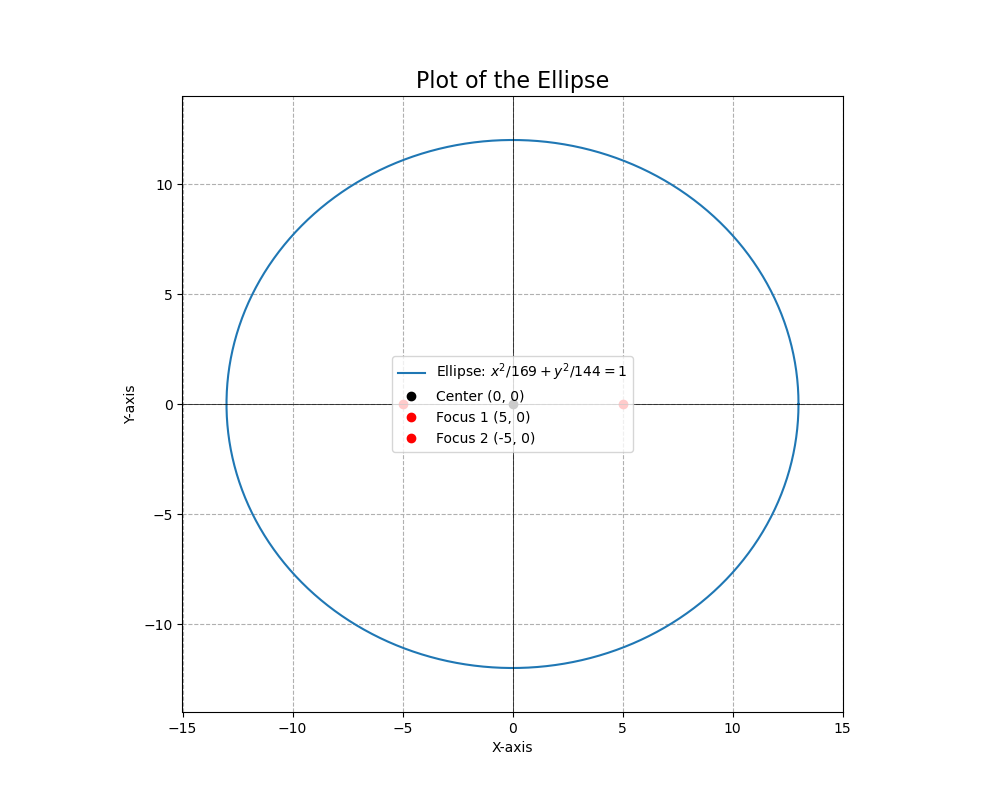
\includegraphics[width=\columnwidth]{figs/fig3.png}
    \end{center}
    \label{fig:Fig.1}
    \end{figure}
\end{frame}    

\end{document}

